\documentclass[../Proposal.tex]{subfiles}
 
\begin{document}
	\section{Perancangan Sistem}
	\subsection{Gambaran Umum Sistem}
	Gambaran umum sistem yang akan dibuat adalah. Sudah didapat informasi mengenai dokumen yang terindikasi \textit{X} plagiat beserta sumbernya \textit{Y}. Kedua dokumen akan di ekstrak dan diambil cirinya dengan metode \textit{N-Gram} lalu membuat \textit{seed} yang akan di bandingkan di proses \textit{merging}. Dari proses \textit{merging} akan dilanjutkan ke proses \textit{filtering} dan mengklasifikasi hasil yang ada kedalam klasifier untuk menentukan jenis tindak plagiat.
	
	\subsection{Alur Sistem}
	Pada kasus sebenarnya, untuk menyusun sistem \textit{Plagiarism Detection} ini membutuhkan 2 \textit{tasks} utama, yaitu \textit{\textbf{Source Retrieval}} dan \textbf{\textit{Text Alignment}}. Sehingga sistem yang seharusnya dibangun ditunjukan oleh gambar \ref{all-sistem}.
	
	\begin{figure}[h!]
		
		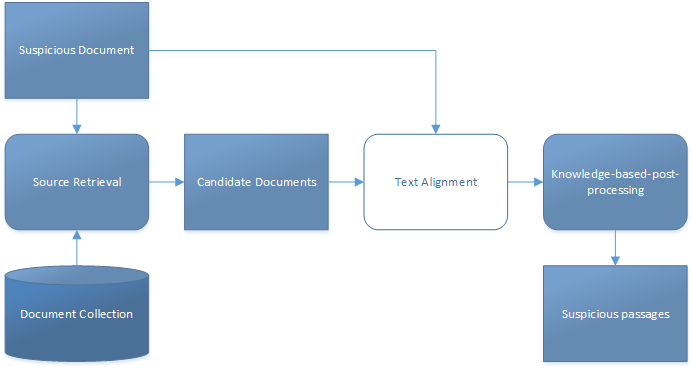
\includegraphics[width=340pt]{SkemaAll}
		\caption[Dataset]{Alur Sistem Keseluruhan}
		\label{all-sistem}
	\end{figure}
	
	Namun, pada tugas akhir ini \textit{Candidate Documents} yang ada pada gambar \ref{all-sistem} sudah didapatkan sebelumnya. Sehingga pada tugas akhir ini akan fokus membahas mengenai \textit{task Text Alignment}. Untuk membuktikan kebenaran dari \textit{Candidate Documents} hasil dari \textit{task Source Retrieval} sebelumnya.\\
	
	Adapun sistem yang akan dibangun ditunjukan oleh gambar \ref{fig:alursistem}.
	
	\begin{figure}[h!]
		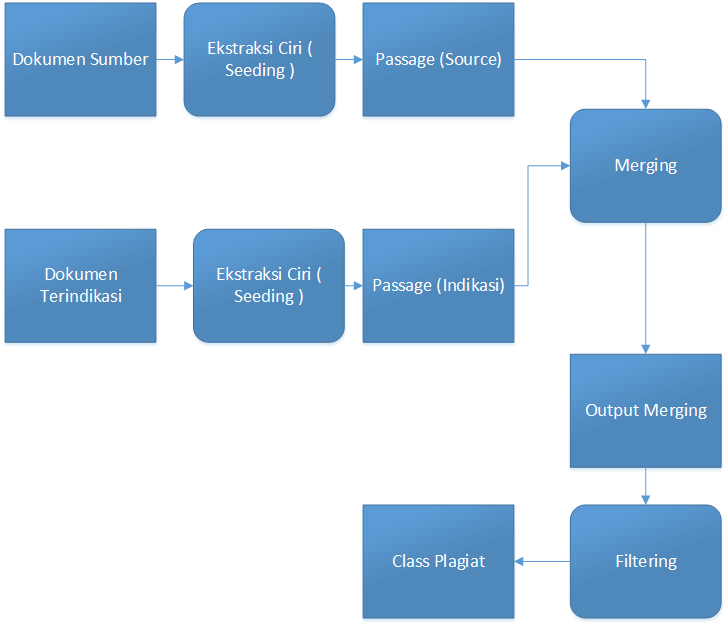
\includegraphics[width=300pt]{Skema2}
		\caption[Alur Sistem]{Alur Sistem}
		\label{fig:alursistem}
	\end{figure}
\end{document}